\documentclass[peerreview]{IEEEtran}
\usepackage{cite}
\usepackage{url}
\usepackage[utf8]{inputenc}
\usepackage{booktabs}
\usepackage{graphicx}
\usepackage[spanish]{babel}
\usepackage{amsmath}
\usepackage{amssymb}
\usepackage{tikz}
\usetikzlibrary{automata,positioning,shapes,arrows,shadows}
\newtheorem{theorem}{Teorema}
\newtheorem{defin}{Definición}
\usepackage{float}
\usepackage{amsmath}
\usepackage{algorithm}
\usepackage{algorithmic}
% traducción
\floatname{algorithm}{Algoritmo}
\renewcommand{\listalgorithmname}{Lista de algoritmos}
\renewcommand{\algorithmicrequire}{\textbf{Entrada:}}
\renewcommand{\algorithmicensure}{\textbf{Salida:}}
\renewcommand{\algorithmicend}{\textbf{fin}}
\renewcommand{\algorithmicif}{\textbf{si}}
\renewcommand{\algorithmicthen}{\textbf{entonces}}
\renewcommand{\algorithmicelse}{\textbf{si no}}
\renewcommand{\algorithmicelsif}{\algorithmicelse,\ \algorithmicif}
\renewcommand{\algorithmicendif}{\algorithmicend\ \algorithmicif}
\renewcommand{\algorithmicfor}{\textbf{para}}
\renewcommand{\algorithmicforall}{\textbf{para todo}}
\renewcommand{\algorithmicdo}{\textbf{hacer}}
\renewcommand{\algorithmicendfor}{\algorithmicend\ \algorithmicfor}
\renewcommand{\algorithmicwhile}{\textbf{mientras}}
\renewcommand{\algorithmicendwhile}{\algorithmicend\ \algorithmicwhile}
\renewcommand{\algorithmicloop}{\textbf{repetir}}
\renewcommand{\algorithmicendloop}{\algorithmicend\ \algorithmicloop}
\renewcommand{\algorithmicrepeat}{\textbf{repetir}}
\renewcommand{\algorithmicuntil}{\textbf{hasta que}}
\renewcommand{\algorithmicprint}{\textbf{imprimir}} 
\renewcommand{\algorithmicreturn}{\textbf{devolver}} 
\renewcommand{\algorithmictrue}{\textbf{cierto }} 
\renewcommand{\algorithmicfalse}{\textbf{falso }} 



\begin{document}
\title{Seguridad de la información en la red basada en el sistema de criptografía AES}


\author{Kevin Alejandro Herrera\\
Escuela de Matemática y Ciencias de la Computación\\
Universidad Nacional Aut\'onoma de Honduras\\
e-mail: kherrerar@unah.hn
}
\date{\today}

\maketitle
\tableofcontents
\listoffigures
\listoftables

\IEEEpeerreviewmaketitle
\begin{abstract}
Será escrito al terminar el proyecto de investigación
\bigbreak 
\textit{Palabras claves:} AES, criptografía, seguridad de la información, cifrado.
\end{abstract}






\section{Introducci\'on}
Será escrito al terminar el proyecto de investigación

\section{Planteamiento del problema}
 El avance tecnológico con el pasar del tiempo ha crecido de manera exponencial, con ello el flujo de información en la red ha aumentado su volumen, por tanto muchos de estos datos se encuentran vulnerables al no tener un sistema de seguridad adecuado que pueda resguardar dichos datos, estos mismos pertenecen a organizaciones, empresas o personas de interés.
 \bigbreak
 A medida avanza la tecnología para bien también avanza para mal y muchos de estos sistemas quedan obsoletos ante ataques cada vez indefendibles, para ello se debe implementar un método de seguridad informática; la criptografía en sus diferentes sistemas ayudará de manera eficiente a proteger esta información.
 \bigbreak
%%%%%%%%%%%%%%%%%%%%%%%%%%%%%%%%%%%%%%%%%%%%%%%%%%%%%%%%%%%%%%%%%%%%%%
  En particular el cifrado simétrico preserva la confidencialidad tanto en las transmisiones de información como en su almacenamiento, protegiendo los archivos y evitando que personas ajenas tengan acceso a la información.


\section{Preliminares y Notaci\'on}
\subsection{Entradas y salidas}
La salida y entrada del algoritmo AES consiste en una secuencia de \textit{128 bits} (dígitos con valores de 0 o 1). Estas secuencias a veces se denominarán \textit{bloques} y el número de
los bits que contienen se denominarán \textit{longitud}.
\subsection{Bytes}
\begin{defin}[Byte]
   Es una cadena de $8$ \textit{bits}, representados como $\{b_7, b_6, b_5, b_4, b_3, b_2, b_1, b_0\}$, estos toman el valor de $0$ o $1$. Es la unidad básica de procesamiento del algoritmo AES.
\end{defin}
\bigbreak
La principal y básica estructura algebraica usada en el sistema AES es el campo binario de Galois $GF(2)$ (llamados \textit{bits}). Por tanto un \textit{byte} se puede representar en un campo finito $GF(2^8)$ utilizando una representación polinomial a través de la fórmula:
$$\sum_{i=0}^{7}b_{i}x^{i}$$

En el algoritmo AES trataremos a los \textit{bytes} en notación hexadecimal, como se puede ver en el cuadro 
\begin{table}[ht]
\centering
\begin{tabular}{|c|c|}
\hline
\textbf{Cadena de bits} & \textbf{Carácter hexadecimal} \\ \hline
0000                    & 0                             \\ \hline
0001                    & 1                             \\ \hline
0010                    & 2                             \\ \hline
0011                    & 3                             \\ \hline
0100                    & 4                             \\ \hline
0101                    & 5                             \\ \hline
0110                    & 6                             \\ \hline
1000                    & 8                             \\ \hline
1001                    & 9                             \\ \hline
1010                    & A                             \\ \hline
1011                    & B                             \\ \hline
1100                    & C                             \\ \hline
1101                    & D                             \\ \hline
1110                    & E                             \\ \hline
1111                    & F                             \\ \hline
\end{tabular}
\caption{Notación hexadecimal}
\label{tab:HEX}
\end{table}
\subsection{Matriz de estado}
El algoritmo AES divide los datos de entrada en bloques de $4$ palabras de $32$ \textit{bits}, decir $4 \times 32 = 128$ \textit{bits}, se puede ver como una sucesión de $16$ \textit{bytes}.\\

Para comprender las operaciones que se realizan en AES, representaremos los $16$ \textit{bytes} como una matriz de $4\times 4$(cuatro filas por cuatro columnas) llamada \textbf{matriz de estado}. Un \textit{byte} se representara por la letra $B$ por tanto nuestra matriz de estado será la siguiente:
$$ \begin{bmatrix}
B_{15} & B_{14} & B_{13} & B_{12} \\
B_{11} & B_{10} & B_9 & B_8 \\
B_7 & B_6 & B_5 & B_4 \\
B_3 & B_2 & B_1 & B_0 
\end{bmatrix}  $$
\subsection{Operaciones matemáticas}
Todos los bytes en el algoritmo de AES son interpretados como elementos de un campo finito, estos elementos pueden sumarse y multiplicarse, pero estas operaciones son diferentes a las que se utilizan con los números usuales.
\bigbreak

\subsubsection{Suma (o resta)}
La suma y resta se caracteriza por tener el mismo resultado y está dado por el operador lógico \textit{or} exclusivo (XOR) bit a bit. Esta operación se representa por el símbolo $\oplus$.

\begin{table}[h]
\centering
\begin{tabular}{|c|c|c|}
\hline
A & B & A $\oplus$ B \\ \hline
0 & 0 & 0         \\ \hline
0 & 1 & 1         \\ \hline
1 & 0 & 1         \\ \hline
1 & 1 & 0         \\ \hline
\end{tabular}
\caption{\label{tab:XOR}Operación XOR.}
\end{table}
\textbf{Ejemplo:}
Consideremos $\{0101 1011\}$ y $\{1101 0110\}$
\begin{itemize}
    \item $01011011 \oplus 11010110=10001101$ (Notación binaria)
    
    \item $5B\oplus D6=8D$ (Notación hexadecimal)
    
    \item $(x^6 +x^4 +x^3 +x+1)\oplus (x^7 + x^6 + x^4 + x^2 +x)=x^7 + x^3 + x^2 +1$ (Notación polinómica)
\end{itemize}

\begin{algorithm}
\begin{algorithmic}[1]
  \REQUIRE $f(x)=\sum_{i=0}^{7}a_{i}x^{i}$, $g(x)=\sum_{i=0}^{7}b_{i}x^{i} \in GF(2^8)$
  \ENSURE  $h(x)=\sum_{i=0}^{7}c_{i}x^i \in GF(2^8)$
  \FOR{$i=0 \text{ hasta } 7$}
  \STATE $c_i  \to (a_i + b_i) \text{ mod } 2$
  \ENDFOR
\end{algorithmic} 
  
  \caption{Algoritmo de la suma en $GF(2^8)$}
  \label{a1}
\end{algorithm}
\subsubsection{Multiplicación}: Se calcula como el residuo de la multiplicación binaria de dos componentes, teniendo en cuenta la suma y resta en campo finito, con el polinomio irreducible \footnote{Un polinomio es irreducible si sus únicos divisores son el mismo y la unidad.} dado por:
    $$m(x)=x^8 + x^4 + x^3 + x +1 $$
    Esta operación se denota por el símbolo $\bullet$.

Para multiplicar dos \textit{bytes} se escribirán en forma polinómica, teniendo en cuenta que la suma es equivalente a una operación XOR. Al realizar la multiplicación es probable que se tenga un resultado de más de $8$ \textit{bits} por tanto se necesitará hacer modulo de dicho polinomio con el polinomio irreducible $m(x)$ para así volver a tener $1$ \textit{byte}. 

\textbf{Ejemplo:} Consideremos $\{01010111\}\bullet\{10000011\}$
\begin{itemize}
    \item $(x^6 +x^4 +x^2 +x^1 + x +1)\bullet(x^7 + x+1)= x^{13} + x^{11} + x^{
    9}+x^{8}+x^{6}+x^5 + x^4 + x^3 +1$
\end{itemize}
Evidentemente este nuevo polinomio no contiene $8$ \textit{bits}, entonces:
$$x^{13} + x^{11} + x^{9}+x^{8}+x^{6}+x^5 + x^4 + x^3 +1 \text{ mod } x^8 + x^4 +x^3 +x +1$$
$$=x^7 + x^6 +1$$ que corresponde a $11000001.$
\begin{algorithm}
\begin{algorithmic}[1]
  \REQUIRE $f(x)=\sum_{i=0}^{7}a_{i}x^{i}$, $g(x)=\sum_{i=0}^{7}b_{i}x^{i} \in GF(2^8)$
  \ENSURE  $h(x)=\sum_{i=0}^{7}c_{i}x^i \in GF(2^8)$
  \STATE $c \leftarrow 0$
  \FOR{$i=0 \text{ hasta } 7$}
  \STATE $c_i  \leftarrow b_i f(x) + c$
  \STATE $f(x) \leftarrow f(x)(x^i) \text{ mod } m(x)$
  \ENDFOR
\end{algorithmic} 
  
  \caption{Algoritmo de la multiplicación en $GF(2^8)$}
  \label{a2}
\end{algorithm}

%%%%%%%%%%%%%%%%%%%%%%%%%%%%%%%%%%%%%%%%%%%%%%%%%%%%%%%%%%%%%%%%%%%%%%








\section{Seguridad Informática}
\begin{defin}[Seguridad de la información]
Conjunto de medidas preventivas de las organizaciones  que permiten resguardar y proteger la información buscando mantener la confidencialidad, disponibilidad e integridad de la misma.
\end{defin}
\bigbreak
Esta seguridad busca la preservación de tres pilares:
\begin{itemize}
    \item La \textit{confidencialidad} es el principio que garantiza que la información solo puede ser accedida por las personas que tienen autorización.
    \item La \textit{integridad} es que la información sólo puede ser creada y modificada por quien esté autorizado a hacerlo.
    \item La \textit{disponibilidad} es que la información debe ser accesible para su consulta o modificación cuando se requiera.
\end{itemize}
\bigbreak
Estos tres conceptos forman lo que a menudo se denomina la tríada CIA. Los tres conceptos encarnan los objetivos fundamentales de seguridad tanto para los datos como para la información y los servicios informáticos.
\begin{figure}[htbp]
\centering
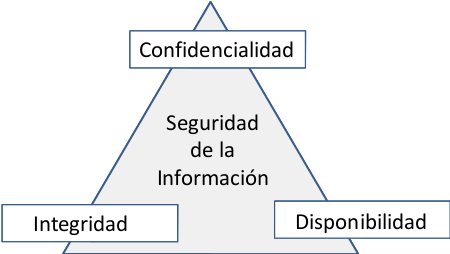
\includegraphics[width=5.5cm]{figuras/cia_tirada.png} 
\caption{Tríada de la CIA}
\label{fig: 1}
\end{figure}
\bigbreak
\begin{defin}[Seguridad informática]
Conjunto de políticas y mecanismos que nos permiten garantizar la confidencialidad, la integridad y la disponibilidad de los recursos en un sistema.
\end{defin}
\bigbreak
\textbf{\textit{Observación:}} El concepto de \textit{seguridad de la información} no debe ser confundido con el de \textit{seguridad informática}, ya que este último sólo se encarga de la seguridad en el medio informático. Sin embargo, la información puede encontrarse en diferentes medios o formas, y no solo en medios informáticos. Es decir que el primer concepto es mas amplio que el segundo.
%%%%%%%%%%%%%%%%%%%%%%%%%%%%%%%%%%%%%%%%%%%%%%%%%%%%%%%%%%%%%%%%%%%%%%
\section{Historia de la criptografía}
La palabra \textit{criptografía} proviene en un sentido etimológico  del griego Kriptos = ocultar, Graphos = escritura, lo que significaría escritura oculta.
\bigbreak
En su clasificación dentro de las ciencias, la \textit{criptografía} proviene de una rama de las matemáticas como se muestra en la figura \ref{fig: 2} que fue iniciada por el matemático Claude Shannon \footnote{Claude Elwood Shannon fue un matemático, ingeniero eléctrico y criptógrafo estadounidense recordado como \textit{el padre de la teoría de la información}}. en 1948, denominada: Teoría de la información.

\begin{figure}[htbp]
\centering
\includegraphics[width=6.5cm]{figuras/origen_criptografía.PNG} 
\caption{Origen de la criptografía.}
\label{fig: 2}
\end{figure}

\begin{defin}[Criptografía]
Ciencia encargada de diseñar funciones o dispositivos, capaces de transformar mensjaes legibles a mensajes cifrados de tal manera que esta transformación (cifar) y su transformación inversa (descifrar) sólo pueden ser factibles con el conocimiento de una o mas llaves.
\end{defin}
\bigbreak
La \textit{criptografía} se puede clasificar en dos: \begin{itemize}
    \item La criptografía clásica
    \item La criptografía moderna
\end{itemize}
%%%%%%%%%%%%%%%%%%%%%%%%%%%%%%%%%%%%%%%%%%%%%%%%%%%%%%%%%%%%%%%%%%%%%%
\section{Advanced Encryption Standard (AES)}
\subsection{Estructura del algoritmo}
La estructura de este algoritmo consiste en una serie de rondas donde se realizan un conjunto de cuatro transformaciones orientadas a \textit{bytes}, el número de rondas depende de la longitud de la llave.

Vamos a asumir que la longitud de la llave escogida es de 128 \textit{bits} ya que la longitud de la llave no afecta a las diversas trasformaciones que realiza el cifrado.
\begin{table}[h]
\centering
\resizebox{9cm}{!}{
\begin{tabular}{l|c|c|c|}
\cline{2-4}
                              & \begin{tabular}[c]{@{}c@{}}\textbf{Longitud de llave}\\ \textit{(Nk words)}\end{tabular} & \begin{tabular}[c]{@{}c@{}}\textbf{Tamaño de bloque}\\ \textit{(Nb words)}\end{tabular} & \begin{tabular}[c]{@{}c@{}}\textbf{Número de rondas}\\ \textit{(Nr)}\end{tabular} \\ \hline
\multicolumn{1}{|l|}{AES-128} & 4                                                                      & 4                                                                     & 10                                                              \\ \hline
\multicolumn{1}{|l|}{AES-192} & 6                                                                      & 4                                                                     & 12                                                              \\ \hline
\multicolumn{1}{|l|}{AES-256} & 8                                                                      & 4                                                                     & 14                                                              \\ \hline
\end{tabular}
}
\caption{Número de rondas en función de la longitud de la llave}
\label{tab:cuadro3}
\end{table}


Básicamente se aplican cuatro trasformaciones a la matriz de estado durante el número determinado de rondas, las cuales se detallaran a continuación.
\bigbreak
\subsubsection{Subbytes()}
Esta operación consiste en una transformación no lineal, donde se realiza una sustitución de cada byte por otro byte establecido en la caja de sustitución (S-box) ver cuadro \ref{tab:cuadro4}.
\begin{figure}[h]
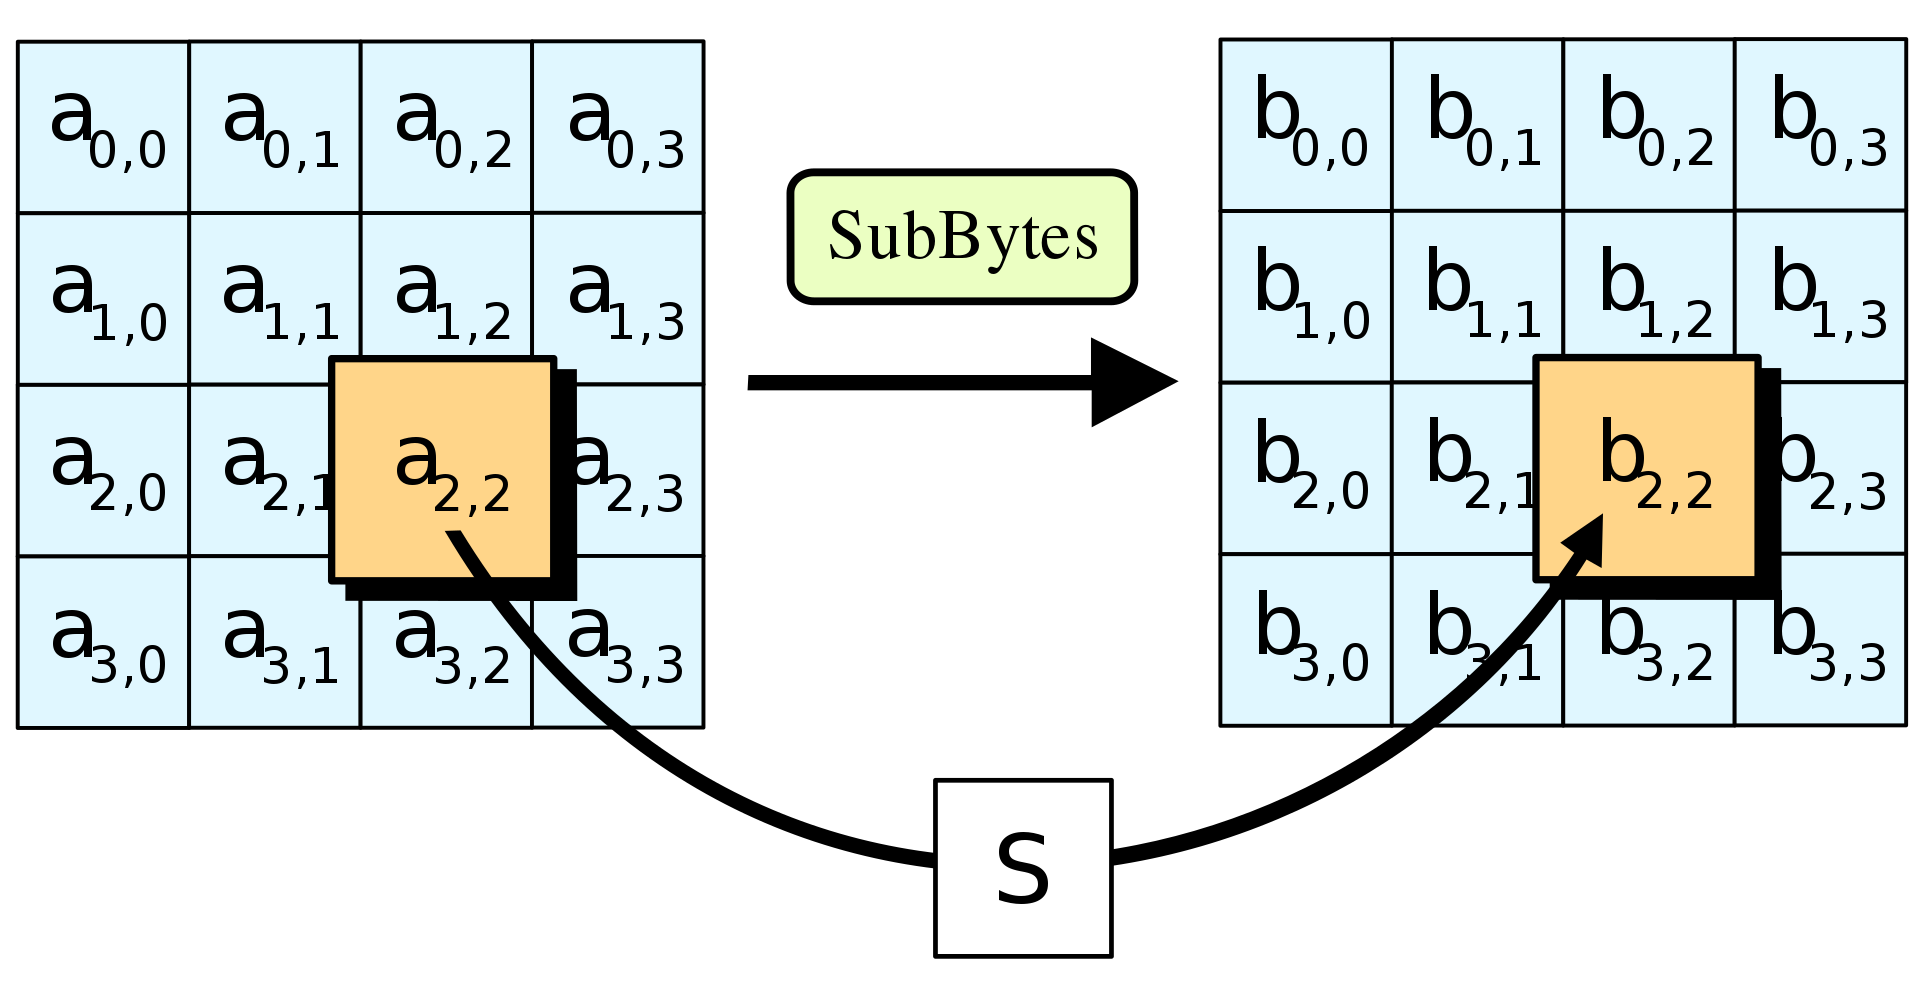
\includegraphics[width=6cm]{figuras/SubBytes.png}
\centering
\caption{Transformación SubBytes}
\label{fig: 3}
\end{figure}

AES define una matriz de valores de \textit{bytes} de $16 \times 16$ llamada S-Box, que contiene una permutación de todos los 256 valores de 8 \textit{bits} posibles.
 \begin{table}[ht]
    \centering
    \resizebox{10cm}{!}{
\begin{tabular}{|c|c|c|c|c|c|c|c|c|c|c|c|c|c|c|c|c|}
\hline
-          & \textbf{0} & \textbf{1} & \textbf{2} & \textbf{3} & \textbf{4} & \textbf{5} & \textbf{6} & \textbf{7} & \textbf{8} & \textbf{9} & \textbf{A} & \textbf{B} & \textbf{C} & \textbf{D} & \textbf{E} & \textbf{F} \\ \hline
\textbf{0} & 63         & 7E         & 77         & 7B         & F2         & 6B         & 6F         & C5         & 30         & 01         & 67         & 2B         & FE         & D7         & AB         & 76         \\ \hline
\textbf{1} & CA         & 82         & C9         & 7D         & FA         & 59         & 47         & F0         & AD         & D4         & A2         & AF         & 9C         & A4         & 72         & C0         \\ \hline
\textbf{2} & B7         & FD         & 93         & 26         & 36         & 3F         & F7         & CC         & 34         & A5         & E5         & F1         & 71         & D8         & 31         & 15         \\ \hline
\textbf{3} & 04         & C7         & 23         & C3         & 18         & 96         & 05         & 9A         & 07         & 12         & 80         & E2         & EB         & 27         & B2         & 75         \\ \hline
\textbf{4} & 09         & 83         & 2C         & 1A         & 1B         & 6E         & 5A         & A0         & 52         & 3B         & D6         & B3         & 29         & E3         & 2F         & 84         \\ \hline
\textbf{5} & 53         & D1         & 00         & ED         & 20         & FC         & B1         & 5B         & 6A         & CB         & BE         & 39         & 4A         & 4C         & 58         & CF         \\ \hline
\textbf{6} & D0         & EF         & AA         & FB         & 43         & 4D         & 33         & 85         & 45         & F9         & 02         & 7F         & 50         & 3C         & 9F         & A8         \\ \hline
\textbf{7} & 51         & A3         & 40         & 8F         & 92         & 9D         & 38         & F5         & BC         & B6         & DA         & 21         & 10         & FF         & F3         & D2         \\ \hline
\textbf{8} & CD         & 0C         & 13         & EC         & 5F         & 97         & 44         & 17         & C4         & A7         & 7E         & 3D         & 64         & 5D         & 19         & 73         \\ \hline
\textbf{9} & 60         & 81         & 4F         & DC         & 22         & 2A         & 90         & 88         & 46         & EE         & B8         & 14         & DE         & 5E         & 0B         & DB         \\ \hline
\textbf{A} & E0         & 32         & 3A         & 0A         & 49         & 06         & 24         & 5C         & C2         & D3         & AC         & 62         & 91         & 95         & E4         & 79         \\ \hline
\textbf{B} & E7         & C8         & 37         & 6D         & 8D         & D5         & 4E         & A9         & 6C         & 56         & F4         & EA         & 65         & 7A         & AE         & 08         \\ \hline
\textbf{C} & BA         & 78         & 25         & 2E         & 1C         & A6         & B4         & C6         & E8         & DD         & 74         & 1F         & 4B         & BD         & 8B         & 8A         \\ \hline
\textbf{D} & 70         & 3E         & B5         & 66         & 48         & 03         & F6         & 0E         & 61         & 35         & 57         & B9         & 86         & C1         & 1D         & 9E         \\ \hline
\textbf{E} & E1         & F8         & 98         & 11         & 69         & D9         & 8E         & 94         & 9B         & 16         & 87         & E9         & CE         & 55         & 28         & DF         \\ \hline
\textbf{F} & 8C         & A1         & 89         & 0D         & BF         & E6         & 42         & 68         & 41         & 99         & 2D         & 0F         & B0         & 54         & BB         & 16         \\ \hline
\end{tabular}
}
\caption{S-box}
\label{tab:cuadro4}
\end{table}

\subsubsection{ShiftRows()}
Esta transformación consiste en una rotación cíclica hacia la izquierda de las filas de la matriz de estado, de manera que la primera fila permanece igual, la segunda fila se rota hacia la izquierda una posición, la tercera fila se rota hacia la izquierda dos posiciones y la ultima fila se rota tres posiciones a la izquierda. 
\begin{figure}[h]
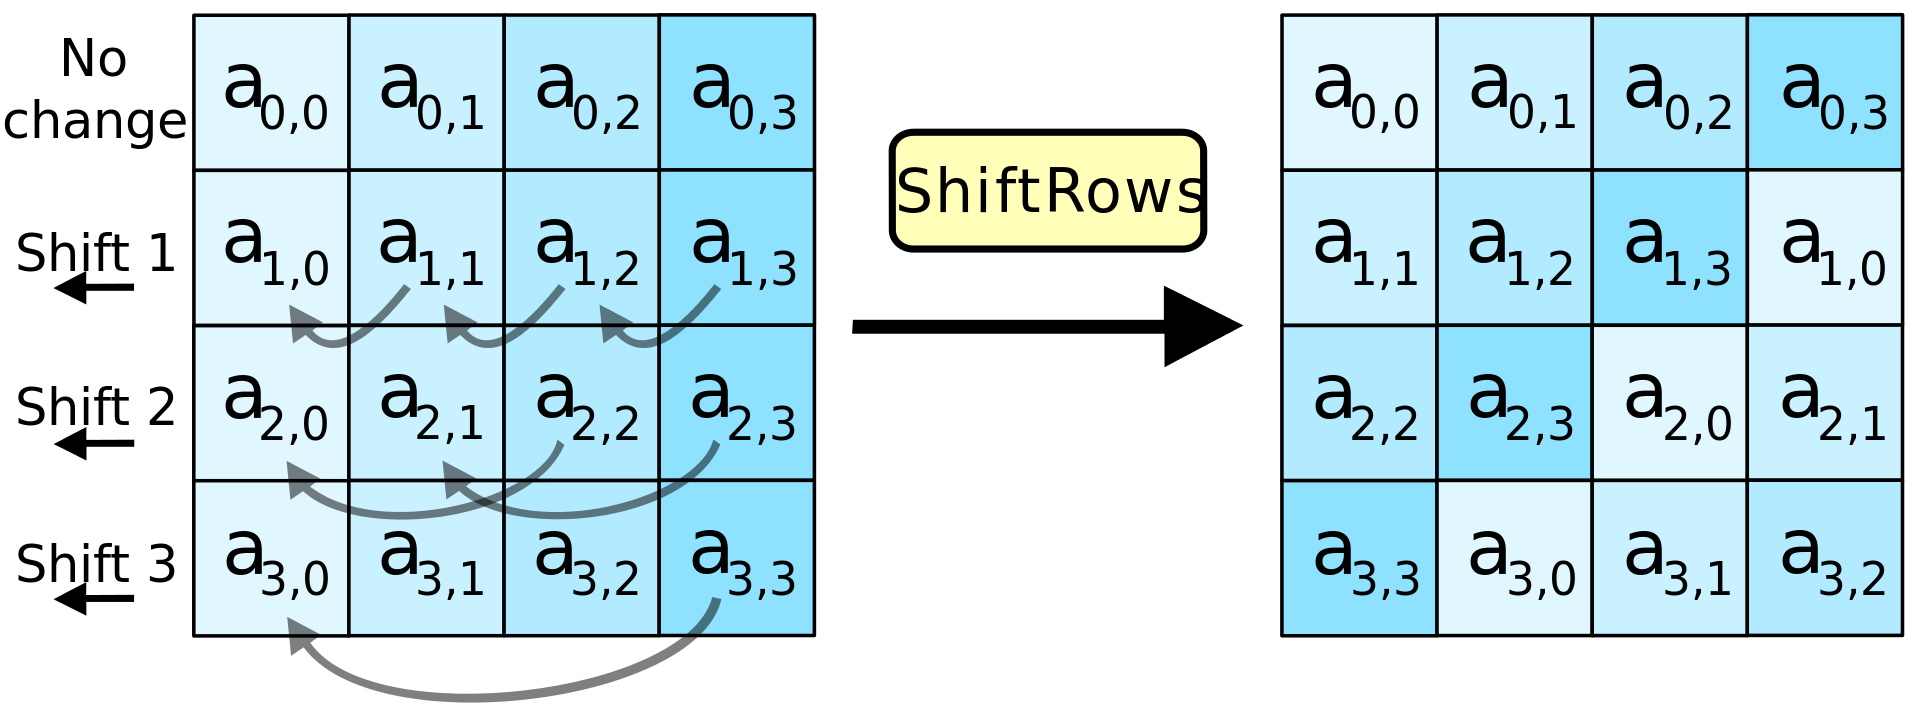
\includegraphics[width=6cm]{figuras/ShiftRows.png}
\centering
\caption{Transformación ShiftRows}
\label{fig: 4}
\end{figure}

\subsubsection{MixColumns()}
Esta trasformación consiste en multiplicar las columnas de bytes módulo $x^4 + 1$ por el polinomio
    $$c(x)=\{03\}x^3 + \{01\}x^2 + \{01\}x + \{02\}$$
    
Es mas sencillo verlo como una multiplicación matricial. Sea:

$$b(x)= c(x)\otimes a(x):$$
$$ \begin{bmatrix}
b_{0, c}\\
b_{1, c}\\
b_{2, c}\\
b_{3, c}\\
\end{bmatrix} = \begin{bmatrix}
02 & 03 & 01 & 01 \\
01 & 02 & 03 & 01 \\
01 & 01 & 02 & 03 \\
03 & 01 & 01 & 02 
\end{bmatrix} \begin{bmatrix}
a_{0, c}\\
a_{1, c}\\
a_{2, c}\\
a_{3, c}\\
\end{bmatrix} \text{para } 0 \leq c \leq \text{\textbf{Nb.}}$$
Los cuatro \textit{bytes} de la columna son reemplazados como se ve a continuación:
$$b_{0, c}=(\{02\}\bullet a_{0, c})\oplus(\{03\}\bullet a_{1, c})\oplus a_{2, c}\oplus a_{3, c}$$
$$b_{1, 0}=a_{0, c}\oplus (\{02\}\oplus a_{1, c})\oplus(\{03\}\bullet a_{2, c})\oplus a_{3, c}$$
$$b_{2, c}= a_{0, c} \oplus a_{1, c} \oplus (\{02\}\bullet a_{2, c})\oplus (\{03\} \bullet a_{3, c})$$
$$b_{3, c}= (\{03 \}\bullet a_{0, c}) \oplus a_{1, c}\oplus a_{2, c} \oplus (\{02\}\bullet a_{3, c})$$
\clearpage
\begin{figure}[ht]
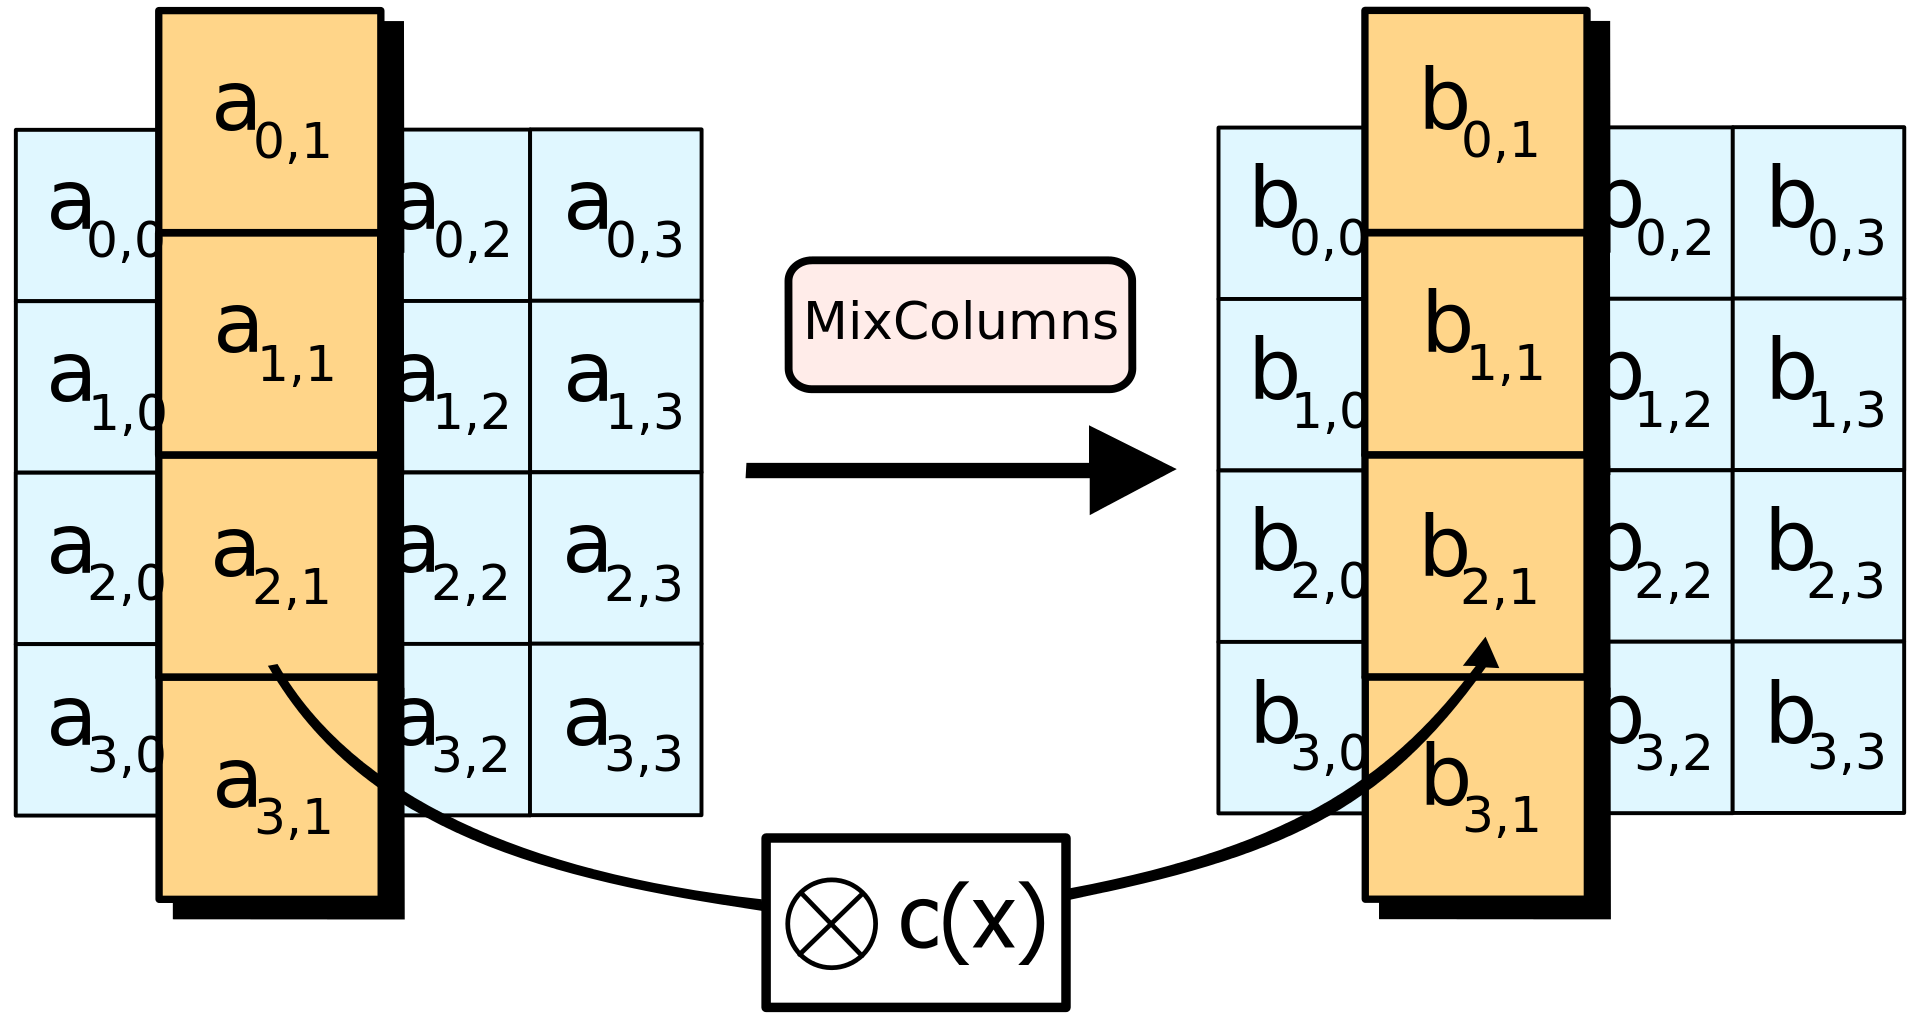
\includegraphics[width=6cm]{figuras/MixColumns.png}
\centering
\caption{Transformación MixColumns}
\label{fig: 5}
\end{figure}´

\subsubsection{AddRoundKey()}
Esta transformación consiste en aplicar la operación OR-Exclusivo (XOR) entre cada byte de la matriz de estado que proviene de la trasformación anterior (MixColumns) y una subclave que se genera a partir de la clave del sistema para esa ronda.
\begin{figure}[ht]
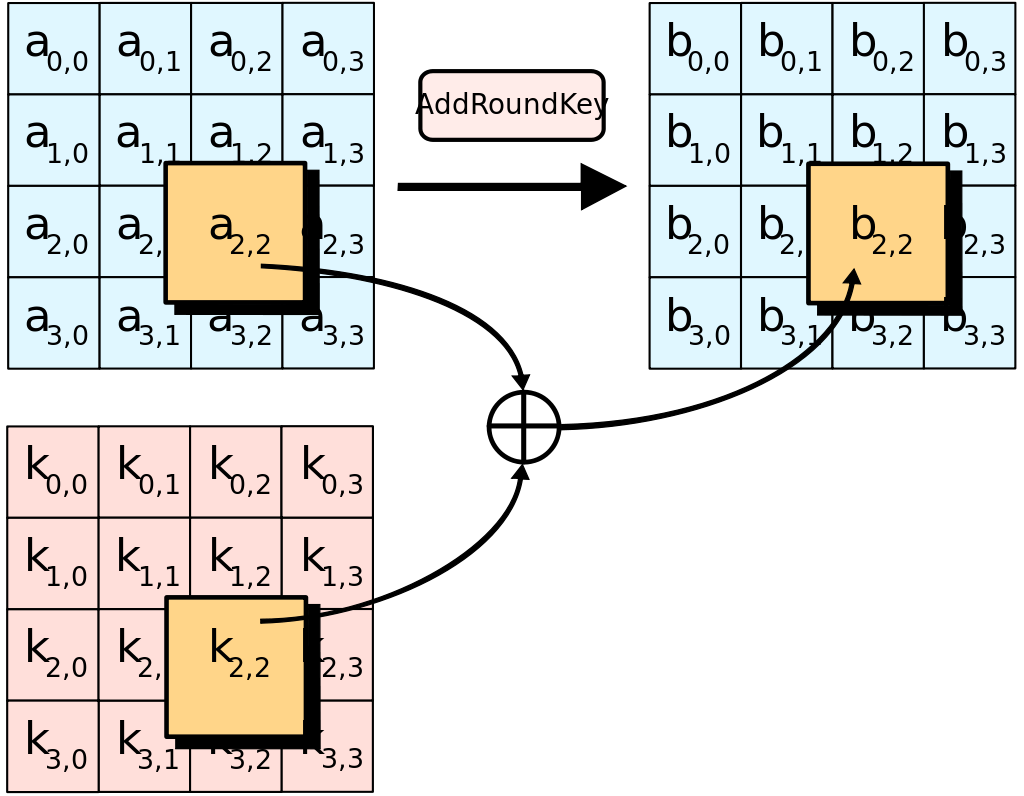
\includegraphics[width=6cm]{figuras/AddRoundKey.png}
\centering
\caption{Transformación AddRoundKey}
\label{fig: 6}
\end{figure}

En la figura que representa el proceso de cifrado (Figura \ref{fig: 7}) esta transformación se realiza en la ronda inicial (ronda 0). Como se definió previamente nuestra longitud de clave será de 128 \textit{bits}, por tanto la subclave de la ronda 0 es la propia clave de cifrado.
\begin{figure}[H]
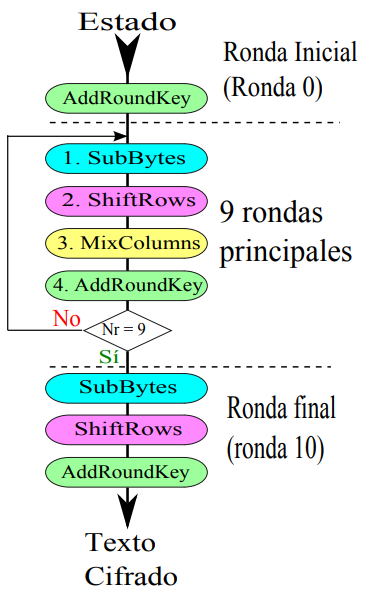
\includegraphics[width=5cm]{figuras/Diagrama1.png}
\centering
\caption{Proceso de cifrado AES}
\label{fig: 7}
\end{figure}
%%%%%%%%%%%%%%%%%%%%%%%%%%%%%%%%%%%%%%%%%%%%%%%%%%%%%%%%%%%%%%%%%%%%%%
 


\section{Trabajo a futuro}

\begin{thebibliography}{1}
\bibitem{Will} \textsc{Stallings, W.} (2016). \textit{Cryptography and Network Security: Principles and Practice} (7.$^{\text{a}}$ ed.). Pearson Education.

\bibitem{Tan} \textsc{Tanenbaum, \& Wheterall.} (2011). \textit{Redes de computadoras} (5.$^{\text{a}}$ ed.). Pearson Education.
\bibitem{tap}\textsc{Tapia-Recillas, H.} (2011). \textit{Sobre algunas aplicaciones de los campos de Galois.} Miscelánea Matemática de la sociedad matemática Mexicana. \url{https://miscelaneamatematica.org/download/tbl_articulos.pdf2.b83a7656c55ef738.353330362e706466.pdf}
\bibitem{NIS01} \textsc{NIST}. (2001). \textit{Announcing the Advanced Encryption Standard (AES)}. Federal Information Processing Standars Publication 197.

\bibitem{GitHub-Docs} GitHub Docs.\textit{ Repositorio proyecto de investigación.} \url{https://github.com/KevinHe23/Proyecto-investigacion}.

\bibitem{GitHub-Docs1} GitHub Docs.\textit{ Repositorio implementación AES.} \url{https://github.com/KevinHe23/Implementacion-AES}.
\end{thebibliography}
\end{document}
